\documentclass{article}
\usepackage[round]{natbib}
\usepackage{listings}
\usepackage[english]{babel}%
\usepackage[T1]{fontenc}%
\usepackage[utf8]{inputenc}%
\usepackage{amsmath,amssymb,amsfonts}%
\usepackage{geometry}%
\usepackage{color}
\usepackage{graphicx}
\usepackage{dsfont}
\usepackage{verbatim}%
\usepackage{environ}%
\usepackage[right]{lineno}%
\usepackage{nameref}
\usepackage{tikz}
%\usepackage{showkeys}

% local definitions
\newcommand{\msprime}[0]{\texttt{msprime}}
\newcommand{\tskit}[0]{\texttt{tskit}}
\newcommand{\ms}[0]{\texttt{ms}}
\newcommand{\scrm}[0]{\texttt{scrm}}
\newcommand{\SLiM}[0]{\texttt{SLiM}}
\newcommand{\fwdpy}[0]{\texttt{fwdpy11}}
\newcommand{\stdpopsim}[0]{\texttt{stdpopsim}}
\newcommand{\SeqGen}[0]{\texttt{Seq-Gen}}
\newcommand{\Pyvolve}[0]{\texttt{Pyvolve}}
\newcommand{\phastsim}[0]{\texttt{phastsim}}

\newcommand{\jkcomment}[1]{\textcolor{red}{#1}}
\newcommand{\plrcomment}[1]{\textcolor{cyan}{#1}}

\begin{document}

\title{Msprime 1.0: an efficient and extensible coalescent simulation framework}
\author{Author list to be filled in
}
% \address{

%%Affiliations:
% Franz Baumdicker:
% Cluster of Excellence "Controlling Microbes to Fight Infections", Mathematical and Computational Population Genetics, University of Tübingen, Germany


% \section*{Contact:} \href{jerome.kelleher@bdi.ox.ac.uk}{jerome.kelleher@bdi.ox.ac.uk}

\maketitle

\begin{abstract}
Coalescent simulation is a key tool in population genetics and
has been integral to coalescent theory since its beginnings.
Because of the ease at which the basic model can be simulated,
a large number of different simulators have been developed. However,
the coalescent with recombination is far more challenging to simulate,
and, until recently, it was not possible to simulate efficiently.
The \msprime\ software has revolutionised
coalescent simulation, making it possible to simulate millions
of whole genomes for the first time. We summarise the many features
of \msprime\ 1.0, which is built around a core model of efficiently
implementing recombination via the succinct tree sequence data
structure. We advocate a community oriented open-source development
process as a way to reduce duplication of effort and increase
the quality of simulation software.
\end{abstract}


\textbf{Keywords:} Coalescent simulation, Python

\section*{Introduction}

The coalescent
process~\citep{kingman1982coalescent,hudson1983testing,tajima1983evolutionary}
models the ancestry of a set of sampled genomes. Given some sampled
genomes, the coalescent provides a mathematical description of the
genealogical tree relating these to each other. Because of its
elegance and simplicity, the coalescent is now central to much of
population genetics and
genomics~\citep{hudson1990gene,hein2004gene,wakely2008coalescent}.
Simulation has been a vital
tool in coalescent theory since its earliest days~\citep{hudson1983testing},
and dozens of different simulation tools have been
developed over the decades~\citep{carvajal2008simulation,liu2008survey,
arenas2012simulation,yuan2012overview,hoban2012computer}.
%% CQ: Reading this sentence, I thought we were still talking abour simulators, that's what I proposed these changes
Two technological developments of recent years, however, have made the majority
of these simulators of little relevance to modern datasets.
% Some citations here? Darwin tree of life maybe?
Firstly, whole genome sequencing ---and in particular fourth-generation
sequencing technologies---have made chromosome-level assemblies
commonplace. Thus, regarding input data as a series of unlinked loci
(a previously reasonable assumption), is no longer defensible and
recombination must be fully accounted for. While the
single-locus coalescent for $n$ samples can be simulated in $O(n)$
time~\citep{hudson1990gene}, the coalescent with recombination is
far more challenging.
% Sentence is too long...
Programs such as Hudson's classical \ms~\citep{hudson2002generating}
can only simulate short segments under the influence of recombination,
and, until recently, approximate models of
recombination~\citep{mcvean2005approximating,staab2015scrm}
were necessary to simulate whole chromosomes.

The second development that has made the majority of
present day simulators inapplicable to modern data sets is the
exponential increase in sample size. Human datasets such
UK Biobank~\citep{bycroft2018genome} and
gnomAD~\citep{karczewski2019variation} now contain hundreds of
thousands of genomes, and there is every reason to believe that
researchers will be soon be routinely working with
datasets containing millions of samples~\citep{stephens2015big}.
Classical simulators such as \ms\ and even fast approximate simulators
such as \scrm\ simply cannot cope with this scale. Even if we
spend months of CPU time on running simulations with millions of samples,
the output would require terabytes of storage space to store and
days of CPU time to parse~\citep{kelleher2016efficient}.

The \msprime\ simulator~\citep{kelleher2016efficient,kelleher2020coalescent}
has greatly increased the scope of coalescent simulations.
Through the use of efficient data structures, it is
now straightforward to simulate millions of whole chromosomes.
The ``succinct tree sequence'' data
structure~\citep{kelleher2016efficient,kelleher2018efficient,kelleher2019inferring,
wohns2021unified},
introduced as part of \msprime\, makes it possible to store simulations
of millions of whole chromosomes in a few gigabytes, several orders
of magnitude smaller than the standard
Newick~\citep{felsenstein1989phylip} or
VCF~\citep{danecek2011variant} based formats.
This data structure has
also lead to major advances in forwards-time
simulation~\citep{kelleher2018efficient,haller2018tree},
ancestry inference~\citep{kelleher2019inferring,wohns2021unified}
and calculation of population genetic statistics~\citep{ralph2020efficiently}.
Through a rigorous open-source community development process,
\msprime\ has gained a large number of features since its introduction,
making a highly efficient and flexible platform for population
genetic simulation.
% This is a bit flat --- anything else to say at the end here?
This paper marks the release of \msprime\ 1.0.

% JK: Earlier notes on this para
% - Msprime 1.0 combines the features of many different simulators and is
%   far more efficient than all of them. The combination of a Python API,
%   an extremely efficient storage format, and a well-engineered and
%   extensible codebase changes the game. Stdpopsim builds on this base
%   to provide easy access to standard models of population genetics.
%

\section*{Results}

\jkcomment{Give a quick roadmap,
like, we discuss the underlying tree sequence object,
then mutations (because it's quite separate from the rest)
and then a bunch of new features for ancestry simulation. There's no
point in listing it out section by section.}

% JK: commented out this text as it's misleading and would confuse
% people. We should adapt it when writing the roadmap when the structure
% has settled down.

% In this section we describe the main features of \msprime\ 1.0. Methodologically,
% there exists a logical separation between simulating coalescent genealogies and
% adding neutral mutations onto these genealogies. Simulating genetic ancestry
% requires methods that model the underlying reproductive process (e.g. Moran,
% Wright-Fisher, etc.) as well as accounting for recombination of various sorts
% (including gene conversion), demography, and selection. These methods are
% discussed in the first N subsections below. One of the strengths of the
% approach taken in msprime is that neutral mutations can be retrospectively
% added to simulated genealogies. Methods to generate mutations, and thereby
% generate genetic variation, are therefore discussed in a separate and subsequent
% subsection. Finally, we describe the \msprime\ API, which is designed to enforce
% the distinction between simulating genealogies and mutations; discuss the
% interoperability provided by the use of \tskit\, the tree sequence toolkit;
% and highlight the open source development process which allows for \msprime\
% to be extended by addition of new features while ensuring robustness and
% maintainability of the core codebase.

\subsection*{Tree sequences}
\label{sec-ts}
One of the key reasons for \msprime's significiant performance advantage
over other simulators~\citep{kelleher2016efficient}
is its usage of the ``succinct tree sequence''
(usually, tree sequence) data stucture
The basic concepts were introduced by \cite{kelleher2016efficient}
and originally developed as part of \msprime. We have subsequently
extracted the tree sequence code from \msprime\ into
\tskit~\citep{tskit2021tskit}, a standalone Python and C library.
While a full discussion of tree sequences and the capabilities
of \tskit\ is beyond the scope of this article, we summarise
the aspects that are important for simulation here.

\begin{figure}
\begin{center}
\includegraphics[width=6cm]{illustrations/example_tree_sequence}
\end{center}
\caption{\label{fig-ts-example} Example tree sequence.
An example tree sequence describing genealogies and genotypes
for four samples at ten sites.
}
\end{figure}

The succinct tree sequence is a data structure for concisely encoding
genetic ancestry and variation. Given a set of sample chromosomes, the topology
of their genetic ancestry is described by a set of \emph{nodes}
and \emph{edges} (Fig.~\ref{fig-ts-example}).
A node in tree sequence terminology corresponds
to a single chromosome strand, and is associated with its birth time,
population and other metadata. A node may optionally be
associated with an \emph{individual}, so that, for example, a diploid
individual will be associated with two separate nodes (we omit
the individual table in Fig.~\ref{fig-ts-example} as it is optional).
Nodes define haplotypes that exist at a specific time within a
some individual, and edges define genetic inheritence
relationships between these nodes. An edge consists of a
parent node, a child node and the left and right coordinates
of the contiguous genomic interval over which
the child inherited genetic material from the parent.
Critically, edges can span multiple marginal trees: for
example, in Fig.~\ref{fig-ts-example} the branch from node
0 to 4 is present in both marginal trees, and represented
by a single edge (the first row in the example edge table).
This simple device, of explicitly associating tree nodes
with specific ancestral chromosomes and recording the
genomic intervals over which parent/child relationships exist,
is a generalisation from the original concept  of
``coalescence records''~\citep{kelleher2016efficient}, and
is the key to the efficiency of tree
sequences~\citep{
kelleher2018efficient,kelleher2019inferring,ralph2020efficiently}.
The term Ancestral Recombination Graph (ARG) is often understood
to mean the complete record of the genetic
ancestry of a set of sampled
genomes~\citep[e.g.][]{mathieson2020ancestry},
and in this sense a tree
sequence \emph{is} an ARG. More technically, an ARG is a particular
graphical representation of genetic ancestry based on the
flow of ancestral material through recombination and common
ancestor events~\citep{griffiths1991two,griffiths1997ancestral}.
In this sense, tree sequences can be used to \emph{encode}
ARGs without loss of information (although we do not store
the additional ARG information by default
in \msprime\ because the minimal tree sequence encoding is
much more concise; see the \nameref{sec-arg} section for more details).
It should be noted that, despite efforts to
standardise~\citep{cardona2008extended,mcgill2013graphml}, there is
no shared format for interchanging ARG data, and no supporting software
libraries.

The point of running simulations is to generate data, and there
are two important ways in which the tree sequences output by
\msprime\ are more useful than classical approaches: (1) tree
sequences are more efficient; and (2) tree sequences contain
more information. We will consider these points in turn.

The classical approach to generating simulation data is
to render the results in some text format. For example,
\ms~\citep{hudson2002generating} outputs a set of sequences
and can also optionally output the marginal trees along
the genome in Newick format,
and variants of this approach are used by many simulators.
Text files have many advantages, but are slow to process
at scale. With sample sizes becoming ever larger, processing
text output can become a significant bottleneck in many analyses.
The ability to efficiently process simulation results is
particularly important in simulation-based inference methods
such as Approximate Bayesian Computation
(ABC)~\citep{beaumont2002approximate,csillery2010approximate,wegmann2010abctoolbox}
and machine learning based
approaches~\citep{sheehan2016deep,chan2018likelihood,schrider2018supervised,
flagel2019unreasonable,sanchez2020deep}. Clearly, simulation efficiency is
crucial since the size and number of simulations that can be performed determines
the depth to which one can sample from the model and parameter space.
Equally important,
however, is the efficiency with which the simulation results can be
transformed into the specific input required by the inference method.
In the case of ABC, this is usually a set of summary statistics of the sequence
data, and methods avoid the bottleneck of parsing
text-based file formats to compute these statistics
by either developing their own
simulators~\citep[e.g.][]{cornuet2008inferring,lopes2009popabc}
or creating forked versions of existing
simulators~\cite[e.g.][]{thornton2006approximate,
hickerson2007msbayes,pavlidis2010msabc,huang2011mtml,quinto2018modeling},
tightly integrated with the inference method.
While this is certainly more efficient,
there is a great deal of duplication of effort and significant
room for error (and propagation of bugs).
Modern approaches to ABC such as
ABC-RF~\citep{raynal2019abc,pudlo2016abc} and
ABC-NN~\citep{csillery2012abc,blum2010abc} use large
numbers of weakly informative statistics,
making the need to efficiently compute statistics from simulation
results even more acute.

Classical text based output formats like \ms\ are inefficient to process,
but also lacking a great deal of important information.
The tree-by-tree topology information output by simulators in Newick
format lacks any concept of node (in the tree sequence sense) identity,
and means that we cannot reliably infer information about ancestors
from the output. Because Newick stores branch lengths rather
than node times, numerical precision issues also arise when summing
over many short branches~\citep{mcgill2013graphml}.
% JK: not sure this is worth leaving in tbh
This lack of reliable information about ancestors in simulation data
has lead, for example, to the definition of segments of
identity by descent as a set of samples having the same time
to their most recent common ancestor along some section of the
genome~\citep{yang2016rapidly}.
Numerous forks
of simulators have been created to access information not provided
in the output. For example, \ms\  has been forked to
output information about migrating segments~\citep{rosenzweig2016powerful},
information about ancestral lineages~\citep{chen2013asymptotic},
an array of population genetic statistics~\citep{ramos2007mlcoalsim}
% Any more?
and \ms's fork \texttt{msHOT}~\citep{hellenthal2007mshot},
has in turn been forked to output information on local
ancestry~\citep{racimo2017archaic}.
All of this information
is either directly available by default in \msprime, or can be optionally
stored via options such as \texttt{record\_migrations} or
\texttt{record\_full\_arg} (see the \nameref{sec-arg} section) and
can be efficiently and conveniently processed via \tskit\ APIs.

\jkcomment{Summary paragraph: tskit gives us complete information
about the genetic ancestry. and is very efficient}

% \jkcomment{A point to make somewhere in here: the tskit data model is
% integrated, with all of the information that you need in one file. Not
% splattered across a number of different files, that you have to keep track
% of.}


\subsection*{Genetic variation}
\label{sec-genetic-variation}

The output of population genetics simulators, quite naturally,
tends to be some representation of the resulting nucleotide sequences
(or some derived statistics of those sequences),
although the underlying genealogies are also of interest.
% Mutations are not treated as first-class data --- the sequences
% were really all people were after, classically.
However, joint information about the mutations that have been simulated
-- e.g., where they have occurred on the trees --
is usually not retained or made available for subsequent analysis.

The approach taken in \msprime\ is quite different.
As illustrated in Fig.~\ref{fig-ts-example}, mutations are an
integral part of \tskit's tree sequence data model, and genetic
variation is encoded by recording sites at which mutations
have occurred, and where each mutation at those sites
has occurred on the marginal tree;
the sequences themselves are never stored.
It may at first seem inconvenient to have only this indirect representation
of the genome sequences, but it is extremely powerful.
Firstly, the storage space required for simulations is dramatically
reduced. For a simulation of $n$ samples with $m$ variant sites,
we would require $O(nm)$ space to store the sequence data as a variant
matrix. However, if this simulation was of a recombining genome
with $t$ trees, then the \tskit\ tree sequence encoding
requires $O(n + t + m)$ space~\citep{kelleher2016efficient},
assuming we have $O(1)$ mutations at each site. For
large sample sizes, this difference is profound, making it
conceivable, for example, to store the genetic ancestry
and variation data for the entire human population on a
laptop~\citep{kelleher2019inferring}. Besides the huge
difference in storage efficiency, it is also often far more efficient
to compute statistics of the sequence data from the
trees and mutations than it is to work with the sequences themselves.
For example, computing Tajima's $D$ from simulated data using \tskit\
is several orders of magnitude faster than efficient variant matrix
libraries for large sample sizes~\citep{ralph2020efficiently}.

The advantages of storing genetic variation data using the underlying trees
have recently become clear in the context of the vast genomic
datasets produced during the SARS-CoV-2 pandemic.
\cite{turakhia2021ultrafast} propose the
Mutation Annotated Tree (MAT)
format (consisting of a Newick tree
and associated mutations in a binary format) and
the \texttt{matUtils} program as an efficient way to store
and process large viral datasets~\citep{mcbroome2021daily},
achieving excellent compression and processing performance.
Similarly, \phastsim~\citep{demaio2021phastsim}
was developed to simulate sequence evolution on such large SARS-CoV-2
phylogenies, and also outputs a Newick tree annotated with mutations (not
in MAT format) to avoid the bottleneck of generating
and storing the simulated sequences.
While these methods illustrate the advantages of the general
approach of storing ancestry and mutations rather than sequences,
they do not generalise beyond their immediate settings, and
no software library support is available.
\msprime, on the other hand, provides a fast, powerful, and well-tested
generic interface for generating and storing mutations on trees.

\subsection*{Simulating mutations}
\label{sec-mutations}

% Explain the background: what have people done classically?
Because coalescent simulations are usually concerned with
neutral evolution (see the \nameref{sec-selection} section, however)
the problem of generating synthetic genetic variation can be decomposed into
two independent steps:
simulating genetic ancestry (the trees), and then simulating
variation by superimposing mutation processes on those trees
(see figure~\ref{fig-mutated-trees}).
A number of programs exist to place mutations on trees:
for instance,
the classical \texttt{Seq-Gen} program~\citep{rambaut1997seq}
allows a range of different models of sequence evolution to be imposed on a given
tree in Newick format, and there are various
extensions to the basic nucleotide
models~\citep[e.g.][]{cartwright2005dna,fletcher2009indelible}.
Population genetic simulators have tended to
include their own implementations of mutation simulation, with
most just supporting the infinite sites
model~\citep[e.g.][]{hudson2002generating}
but with several supporting a range of different models
of sequence
evolution~\citep[e.g.][]{mailund2005coasim,excoffier2011fastsimcoal,
virgoulay2021gspace}.

\begin{figure}
    \includegraphics{illustrations/unmutated_tree}
    \includegraphics{illustrations/mutated_tree}
    \caption{
        \label{fig-mutated-trees}
        Visualization of the separation between ancestry and mutation simulation:
        \texttt{sim\_ancestry} produces ancestry
        (\textbf{left;} shown are two trees along a 1Kb chunk of genome
        relating 200 samples),
        and \texttt{sim\_mutations} adds mutations
        (\textbf{right;} fourteen nucleotide mutations have been added).
        Graphics produced with \tskit's \texttt{draw\_svg} method.
        \plrcomment{TODO: fix up the axis labels, if we like this figure?}
    }
\end{figure}

% on the other hand, tskit is awesome.
Clean separation of the ancestry and mutation generation steps
is made possible by the \tskit\ library, whose mature and
efficient C and Python interfaces makes it straightforward to add
further information to an existing file, and to output the results.
As such, it is essentially a historical accident
that \msprime\ (whose main focus is on ancestry simulation)
contains code to simulate mutations: the mutation process could
be performed by a separate package, and there would be no performance
penalty for doing so.
Thanks to this interoperability, \msprime's
mutation generator can work with \emph{any} \tskit\ tree sequence,
be it simulated using \SLiM~\citep{haller2019slim} or
\fwdpy~\citep{thornton2014cpp}, or estimated from real data
using~\texttt{tsinfer}/\texttt{tsdate}~\citep{kelleher2019inferring,wohns2021unified}
or \texttt{Relate}~\citep{speidel2019method}. It is a modular
component intended to fit into a larger software ecosystem, and
is in no way dependent on \msprime's ancestry simulator.

For version 1.0 we have greatly extended the sophistication of
\msprime's mutation generation engine, achieving near feature-parity
with \SeqGen.
We  support a large number of mutation models, including
JC69~\citep{jukes1969evolution},
F84~\citep{felsenstein1996hidden},
and GTR~\citep{tavare1986some} nucleotide models
and the BLOSUM62~\citep{henikoff1992amino}
and PAM~\citep{dayhoff1978} amino acid models.
A general model accepts an arbitrary transition matrix between
any number of alleles (which can be arbitrary unicode strings),
and so other models such as the Kimura two and three
parameter models~\citep{kimura1980simple,kimura1981estimation}
can be easily and efficiently defined in user code.
Mutation rates can vary along the genome, and multiple mutation
models can be imposed on a tree sequence by overlaying mutations
in multiple passes.
The new \texttt{sim\_mutations} function
(see the \nameref{sec-sim-interface} section) defaults to a finite-sites
mutation model, but full support for the
original infinite sites model is also maintained.
We have extensively validated the results of mutation simulations
against both theoretical expectations and output from
\SeqGen~\citep{rambaut1997seq} and
Pyvolve~\citep{spielman2015pyvolve}.

\begin{figure}
    \includegraphics[width=\textwidth]{figures/mutations-perf}
\caption{\label{fig-mutations-perf} Time required to run
\texttt{sim\_mutations} on tree sequences generated
by \texttt{sim\_ancestry} (with a population size of $10^4$
and recombination rate of $10^{-8}$) for varying (haploid) sample
size and sequence length. We run 10 replicate mutation simulations
each for three different mutation rates, and report the average
CPU time required (Intel Core i7-9700).
(A) Holding sequence length fixed at 10 megabases and varying the
number of samples (tree tips) from 10 to 100,000.
(B) Holding number of samples fixed at 1000, and varying the sequence
length from 1 to 100 megabases.}
\end{figure}

Generating simulations in \msprime\ is extremely efficient.
Fig.~\ref{fig-mutations-perf} shows the time required to generate
mutations (using the default JC69 model) on
simulated tree sequences for a variety of mutation
rates as we vary the number of samples
(Fig.~\ref{fig-mutations-perf}A) and the sequence
length (Fig.~\ref{fig-mutations-perf}B).
For example, the longest running simulation in
Fig.~\ref{fig-mutations-perf}B required less than 2 seconds to
generate an average of 1.5 million mutations over 137,081 trees
in a tree sequence with 508,125 edges.
This efficiency for large numbers of trees is possible because
the tree sequence encoding allows us to generate mutations
on an edge-by-edge basis
(see Fig.~\ref{fig-ts-example} and Appendix~\ref{app-mutation-algorithm}),
rather than tree-by-tree and branch-by-branch as would otherwise be required.
In the above example from Fig.~\ref{fig-mutations-perf}B,
we would have to consider 273,887,838 branches
since there are 137,081 trees and 1,998 branches in each
tree ($\sim500$ times more work).

% python3 evaluation/generate_mutations_perf_data.py benchmark-single-tree
Even if we consider a single tree, \msprime\ generates mutations
extremely efficiently.
For example, we simulated mutations under the BLOSUM62 amino
acid model for a tree with $10^6$ leaves over $10^4$ sites (resulting
in $\sim$260,000 mutations) in about $0.8$ seconds, including
the time required for file input and output.
We do not attempt a systematic benchmarking of \msprime's
mutation generation code against other methods because at this scale it is
difficult to disentangle the effects of inefficient input and
output formats from the mutation generation algorithms.
It seems quite unlikely, however,
that generating mutations with \msprime\ would be a bottleneck in any
realistic analysis.

There are many ways in which the mutation generation code
in \msprime\ could be extended by adapting existing methods.
For example, we hope to add support for
microsatellites~\citep{mailund2005coasim},
codon models~\citep{arenas2007recodon}
and indels~\citep{cartwright2005dna,fletcher2009indelible}.

\subsection*{Recombination}

Recombination is implemented in \msprime\ using Hudson's algorithm, which
works backwards in time tracking the
effects of common ancestor and recombination
events~\citep{hudson1983properties,hudson1990gene,kelleher2016efficient}.
Common ancestor events combine the ancestral material of two lineages, and may
result in coalescences in the marginal trees. Recombination events
split the ancestral material for some lineage, creating two independent
lineages. Using the appropriate data structures~\citep{kelleher2016efficient},
this process is much more efficient to simulate than either
methods based on the Ancestral Recombination Graph
formulation~\citep{griffiths1991two,griffiths1997ancestral}
or the left-to-right approach~\citep{wiuf1999recombination,wiuf1999ancestry}.
In \msprime\ 1.0 recombination rates can vary along a chromosome, allowing
us to simulate recombination hotspots like \texttt{msHOT}~\citep{hellenthal2007mshot}
and empirical recombination maps similar to other
simulators~\citep[e.g.][]{shlyakhter2014cosi2}.
The implementation of recombination in \msprime\ is extensively validated
against analytical results~\citep{hudson1983properties,kaplan1985use}
and results from \ms.

The Sequentially Markovian Coalescent (SMC) is an approximation of the
coalescent with recombination
model~\citep{mcvean2005approximating,marjoram2006fast},
and was originally motivated to a significant degree by the need to
simulate longer genomes than was possible using tools like \ms.
The SMC is a good approximation to the
coalescent with recombination when we have four or fewer sampled
genomes~\citep{hobolth2014markovian,wilton2015smc}, but the
effects of the approximation are less well understood for larger
sample sizes and several approaches have been proposed to
allow simulations that more closely approximate the coalescent
with recombination~\citep{chen2009fast,wang2014new,staab2015scrm}.
The SMC is an important analytical approximation
and has allowed the development of numerous inference
methods~\citep{
li2011inference,
harris2013inferring,
sheehan2013estimating,
schiffels2014inferring,
carmi2014renewal,
rasmussen2014genome,
zheng2014bayesian,
terhorst2017robust}.

\begin{figure}
\begin{center}
    \includegraphics{figures/ancestry-perf}
\end{center}
\caption{\label{fig-ancestry-perf}
    Approximate run time for \msprime\ simulations,
    for \textbf{(left)} small, and \textbf{(right)} larger simulations.
    Each point is the runtime of one simulation,
    for various values of effective population size ($N$),
    genome length ($L$), and number of samples.
    Runtime scales quadratically with the product of $N$ and $L$;
    since recombination rate in these simulations was $10^{-8}$,
    the scaled recombination rate here is $\rho = NL/10^8$,
    shown on the horizontal axis.
    The black line is a quadratic fit separately in each panel.
}
\end{figure}

In human-like parameter regimes, \msprime's implementation of the
exact coalescent with recombination comprehensively outperforms
all other simulators, including those based on SMC
approximations~\citep{kelleher2016efficient}. However, it is important
to note that although the implementation of Hudson's algorithm is
very efficient, it is still quadratic in the scaled recombination rate
$\rho = 4 N_e L$, where $L$ is the length of the genome in units of recombination distance.
This is because Hudson's algorithms tracks recombinations not only
in segments ancestral to the sample, but also between ancestral segments.
Estimates of the number of such ``trapped'' recombinations grow quadratically
with genome length \citep[Eq.~5.10]{hein2004gene}.
Because they do not track such recombinations, efficient SMC implementations
will be faster than \msprime\ for sufficiently high recombination rate,
genome length, or $N_e$. %Until we decide to approximate the recombination process
%between distant ancestral segment. Hint hint.

% \jkcomment{We want to round out this discussion here by giving some
% sort of rough argument for why Hudson's algorithm is quadratic, and discussing
% to Fig.~\ref{fig-ancestry-perf} to show roughly what we can expect
% to simulate in how long. See issue 28.}

Figure~\ref{fig-ancestry-perf} gives a rough idea of the runtime of
a given simulation of a constant size population,
and verifies that runtime scales quadratically with $\rho$,
(\citet{hein2004gene} gives an equation
including the effects of sample size --
see Appendix~\ref{app-theoretical-runtime}.)
and depends much less strongly on the number of samples.
Taking a typical chromosome to be 1 Morgan in length,
these plot show, roughly, that simulating
samples from a population of thousands of individuals takes seconds,
while samples from a population of tens of thousands takes minutes.

However, what about a simulation with \emph{changing} size?
To understand how runtime depends on demography
it helps to consider \emph{why} runtime is quadratic in $\rho$.
At any point in time, \msprime\ must keep track of some number of lineages,
each of which contains some number of chunks of genetic material.
Common ancestor events reduce the number of lineages,
and recombination events increase their number.
However, with long genomes
only a small fraction of the common ancestor events
will involve overlapping segments of ancestry,
and lead to coalescence in the marginal trees.
Such disjoint segments are often far apart (on average, about distance $L/2$),
and so recombine apart again immediately;
it is these large numbers of rapid yet inconsequential events that lead to the quadratic runtime.
\plrcomment{(this is discussed also in the ARG section; check for overlap)}
The maximum number of lineages occurs when
the increase and decrease in numbers of lineages due to
common ancestor and recombination events balance out;
to get an idea of runtime we can estimate when this occurs.
Suppose that the maximal number of lineages is $M$;
at this time the rate of common ancestor events is $M (M-1) / (4 N_e)$
and the total rate of recombination is $M \ell$,
where $\ell$ is the mean length of genome carried by each lineage
(including ``trapped'' non-ancestral material).
It is known that the maximum number of lineages is reached very quickly \citep{nelson2020accounting},
and at this maximum, recombination and coalescence rates are equal,
so many (roughly half) of these lineages have at least two distant segments of ancestral material
separated by a long segment of genome, implying that $\ell \approx L / 4$.
This implies that $M$ is roughly $L N_e$.
Now, the number of linages decreases gradually, on the coalescent time scale -- so, over roughly $2 N_e$ generations.
Since the total rate of events when there are the maximum number of lineages
happens at rate roughly $L^2 N_e / 4$,
then the total number of events is proportional to $(L N_e)^2$ -- i.e., proportional to $\rho^2$,
as desired.
What does this tell us about time-varying population sizes?
The argument above implies that the work is spread out relatively evenly on the coalescent time scale:
in other words,
more events happen in the time period from 0 to $N_e/2$ generations
than from $N_e/2$ to $N_e$ generations,
but the runtime is not dominated but the more recent time period.

Putting this together:
suppose that population size today is $N_1$,
while longer ago than $T$ generations ago it was $N_2$:
does the runtime depend more on $4 N_1 L$ or $4 N_2 L$?
The answer depends on how $T$ compares to $N_1$: if $T/N_1$ is large,
then runtime will be similar to a population of size $N_1$;
while if $T/N_1$ is small, it will be similar to a population of size $N_2$.
For instance, in many agricultural species $N_1 \propto 100$, while $N_2 \propto 10^5$,
and the runtime will depend critically on $T$ -- in other words,
simulation will be quick in a species with a strong domestication bottleneck,
and slow otherwise.
In practice, we recommend that users estimate runtime by
measuring runtime in a series of simulations with short genome lengths,
possibly varying other parameters to check for interactions,
and then predict runtime by fitting a quadratic curve to genome length.
There is only a weak dependency on sample size
-- notice that in Figure~\ref{fig-ancestry-perf} increasing sample size 100-fold
only increases runtime by a factor of 2 or so.


The SMC~\citep{mcvean2005approximating} and
SMC'~\citep{marjoram2006fast} models are available
in \msprime\ 1.0. However, they are currently implemented using a
naive rejection sampling approach, and are somewhat slower
to simulate than the exact coalescent with recombination. These
models are therefore only appropriate for studying the SMC approximations
themselves; an important avenue for future work is to implement
efficient SMC-like models, perhaps based on the approaches used
in \texttt{cosi2}~\citep{shlyakhter2014cosi2}, to facilitate
simulation of organisms such as \textit{Drosophila melanogaster}.


\subsection*{Gene conversion}

%introduction
Gene conversion is a unidirectional transfer of a short segment of genetic material,
for example between homologous chromosomes~\citep{chen2007gene}.
%description of ancestral process
Just as recombination, gene conversion events split the ancestral material
for some lineage, creating two independent lineages.
In contrast to the previously described recombination process, where the ancestral
material to the left and right of a recombination breakpoint follows two
different ancestral lineages, gene conversion events distribute the genetic material
of a short segment to one ancestral lineage and the part to the left and right of this
segment to another lineage.
%Franz Baumdicker: Not sure if this next sentence is necessary,
% but it might be of interest for some people?
The resulting distribution of ancestral material after a gene conversion event
equals the distribution after two recombination events at the left and right position
of the gene conversion tract, followed by a common ancestor event.
%Impact on LD
However, gene conversions impact much shorter segments than crossover recombinations,
typically below 1kb, and thus affect linkage patterns differently than
recombinations~\citep{korunes2017gene}.

% other simulators
Hudson's \ms\ optionally includes gene conversion and so does
MaCS~\citep{chen2009fast}, while scrm~\citep{staab2015scrm} does not
support gene conversions.
As bacterial recombination can be modeled analogously to eukaryotic allelic
gene conversion, simulators for microbial evolution often include gene conversion
instead of recombination.
This includes the backward simulator SimBac~\citep{brown2016simbac},
the SMC based approach used in FastSimBac~\citep{demaio2017the},
and forward in time tools within the SLiM framework~\citep{cury2020simulation}.

In \msprime\ 1.0 we implemented the coalescent with gene conversion as defined by
\cite{wiuf2000coalescent}, where gene conversion events are initiated between any
two sites in the sequence at a constant (scaled) rate $\gamma$ and
the length of the transferred segment is given by a geometric distributed
random variable with mean length $L$.
% Above I used the discrete case, but we could easily switch to a description for the
% continuous case.
We have implemented this model of gene
conversion in \msprime\ 1.0, and validated the output against
\ms\ and analytical results~\citep{wiuf2000coalescent}.

\begin{figure}
\begin{center}
\includegraphics[width=7cm]{figures/gc-perf}
\end{center}
\caption{\label{fig-gc-perf}Comparison of the running time
for E-coli simulations using \msprime\ and SimBac for varying
sample sizes. The parameters used are chosen to mimic the simulation
of \textit{E. coli} genomes. The genome length was set to 4.5 mb, the scaled per site
gene conversion rate was set to $N_e g = \gamma = 0.015$ and
the mean gene conversion tract length was set to $L = 500$, which is close to
estimated parameters for \textit{E.\ coli}, i.e.\ an effective populations size
$N_e = 1.8e^8$ and a per site per generation conversion rate $g = 8.9e^{-11}$
with mean tract length $L = 542$~\citep{lapierre2016the}.}
\end{figure}

Gene conversion is particularly useful to model homologous recombination in
bacterial evolution,
so we compare the performance of \msprime\ with gene conversion to
SimBac~\citep{brown2016simbac}, a simulator developed specifically to
simulate bacterial evolution. Although \msprime\ is missing some features
relevant to this case, e.g.\ the simulation of circular genomes, it is far
more efficient at simulating the basic processes.
Furthermore, gene conversion can be considered in combination
with other current and future features of \msprime\ 1.0,
including varying recombination rates and complex demographies.

An important avenue for future work
will be to add further features to model bacterial
evolution. In particular, we aim to include bacterial gene transfer and utilize
the succinct tree sequence structure to represent the resulting ancestral gene
transfer graph~\citep{baumdicker2014AGTG}.

\subsection*{Demography}
% TODO should we put in some citations here for the models? Hardly seems
% necessary.
One of the key applications of population genetic simulations is to generate
data for complex demographies. Beyond idealised cases such as stepping-stone or
island models, or specialised cases such as isolation-with-migration models,
analytical results are rarely possible. Simulation is therefore integral to the
development and evaluation of methods for demographic inference. The demography
model in \msprime\ is directly derived from the approach used in \ms, and
supports an arbitrary number of randomly mating populations exchanging migrants
at specified rates. A range of demographic events are supported, which allow for
varying population sizes and growth rates, changing migration rates over time,
as well as population splits, admixtures and pulse migrations.
The location of sampled lineages
can be tracked through time in as much detail as required: each tree node is
automatically associated with the population in which it arose, the location of
lineages can be recorded at any given time via census events, or every lineage
migration can be recorded.

A major change for \msprime\ 1.0 is the introduction of the new Demography API,
designed to address a serious flaw in the \msprime\ 0.x interface which lead to
a number of avoidable errors in downstream
simulations~\citep{ragsdale2020lessons}. Briefly, the 0.x API required three
separate parameters be provided to the \texttt{simulate} function to describe a
demographic model, making it easy to accidentally omit information. The 1.0 API
resolves this issue by creating a new \texttt{Demography} class, which
encapsulates all information about the demographic model, and fully decouples
the definition from other simulation details. An instance of this class is then
provided as a parameter to the new \texttt{sim\_ancestry} function,
substantially reducing the potential for error.
Another improvement over the
0.X APIs is the introduction of explicit population split and admixture events,
and a population state machine that ensures that lineages cannot migrate into
(or be sampled from) inactive populations. This demography model is compatible
with the Demes standard~\citep{gower2021demes}, and the \texttt{Demography}
class supports importing and exporting Demes models.
Models previously constructed using the 0.x API can be seamlessly imported into
the \texttt{Demography} class, and we also support importing demographic
models in the form of Newick species tree descriptions, as well as those
produced by programs such as *BEAST~\citep{heled2009bayesian}.

The \texttt{DemographyDebugger} can output detailed information for debugging
demographic models, but also provides
methods to compute a suite of numerical predictions about the location of
lineages over time, for example the coalescence rates for two or more lineages
drawn from populations at specified times in the past.
Many popular approaches in population genetics use the distribution of
coalescence rates between pairs of lineages in one or more populations to infer
effective population sizes over
time~\citep{li2011inference,sheehan2013estimating,schiffels2014inferring} or
split times and subsequent migration rates between
populations~\citep{wang2020tracking}.
The \texttt{DemographyDebugger} provides a valuable
ground-truth when evaluating such inference methods, as illustrated by
\cite{adrion2020community}.

\subsection*{Instantaneous bottlenecks}

A common approach to modelling the effect of demographic history on genealogies
is to assume that effective population size ($N_e$) changes in discrete steps
which define a series of epochs~\citep{griffiths1994sampling, marth2004allele,
keightley2007joint,li2011inference}. In this setting of piecewise constant
$N_e$, capturing a population bottleneck requires three epochs: $N_e$ is
reduced by some fraction $b$ at the start of the bottleneck, $T_{start}$, and
recovers to its initial value at time $T_{end}$~\citep{marth2004allele}. If
bottlenecks are short both on the timescale of coalescence and mutations,
there may be little information about the duration of a bottleneck
($T_{end}-T_{start}$) in sequence data. Thus a simpler, alternative model is to
assume that bottlenecks are instantaneous ($T_{end}-T_{start} \rightarrow 0$)
and generate a sudden burst of coalescence events (a multiple merger event) in
the genealogy. The strength of the bottleneck $B$ can be thought of as an
(imaginary) time period during which coalescence events are collapsed,
i.e.\ there is no growth in genealogical branches during $B$ and the probability that a
single pair of lineages entering the bottleneck coalesce during the bottleneck
is $1-e^{-B}$. Although this simple two parameter model of bottlenecks is
attractive and both analytic results and empirical
inference~\citep{griffiths1994sampling, galtier2000detecting,
bunnefeld2015inferring} have been developed under this model, there has
been no software available to simulate data under instantaneous
bottleneck histories.

We have implemented instantaneous bottlenecks in \msprime~1.0
using a variant of Hudson's linear time single-locus coalescent
algorithm~\citep{hudson1990gene}. Instantaneous bottlenecks are specified
by adding events to the Demography object (see the Demography section)
and can be used in combination with any other demographic modelling
features. We have validated the results of these simulations by comparing
against analytical expectations for coalescence times and the
site frequency spectrum~\citep{bunnefeld2015inferring}.

\subsection*{Multiple merger coalescents}

Kingman's coalescent assumes that only two ancestral lineages can merge at
each merger event. Although this is generally a reasonable approximation there
are certain situations in which the underlying mathematical assumptions are
violated. For example in certain highly fecund organisms
\citep{hedgecock_94,B94,HP11,A04,irwin16}, where individuals have the ability
to produce numbers of offspring on the order of the population size and
therefore a few individuals may produce the bulk of the offspring in any given
generation~\citep{hedgecock_94}. These population dynamics violate basic
assumptions of the Kingman coalescent, and are better modelled by
`multiple-merger' coalescents \citep{DK99,P99,S99,S00,MS01}, in which more than
two lineages can merge in a given event. Multiple-merger coalescent processes
have also been shown to be relevant for modeling the effects of selection on
gene genealogies \citep{Gillespie909,DS04}.

Although multiple merger coalescents have been of significant theoretical
interest for around two decades, there has been little practical software
available to simulate these models.
\cite{kelleher2013coalescent,kelleher2014coalescent} developed packages to
simulate a related spatial continuum model~\citep{barton2010new},
\cite{zhu2015hybrid} simulate genealogies within a species tree
based on a multiple-merger model, and
\cite{becheler2020occupancy} provide a general method for simulating
multiple merger processes
as part of the Quetzal framework~\citep{becheler2019quetzal}.
The \texttt{Beta-Xi-Sim} simulator~\citep{koskela2018multi,koskela2019robust}
includes a number of extensions to the Beta-coalescent.
None of these methods work with large genomes, and very little work
has been performed on simulating multiple merger processes with recombination.

We have added two multiple merger coalescent models in \msprime\ 1.0, the
Beta-coalescent and ``dirac''-coalescent, allowing us to simulate
such models with recombination efficiently for the first time.
These simulation models have been extensively validated against
analytical results from the site frequency
spectrum~\citep{birkner2013statistical,blath2016site,hobolth2019phase}
 as well as more general properties of coalescent processes.
Please see the Appendix for more details and model derivations.

\subsection*{Ancestral Recombination Graphs}
\label{sec-arg}

The Ancestral Recombination Graph (ARG) was introduced by
Griffiths~\citep{griffiths1991two,griffiths1997ancestral} as a graphical
representation of the coalescent with recombination stochastic process. This
formulation was complementary to Hudson's earlier
work~\citep{hudson1983properties}, and substantially increased our theoretical
understanding of recombination. In Griffiths' ARG formulation, we
regard a realisation of the coalescent with recombination as a graph in which
vertices represent common ancestor or recombination events, and edges represent
lineages through which ancestral material flows.
We may consider the big ARG, in which we track lineages arising out of
recombinations regardless of whether they carry ancestral material and
consequently wait an exponentially large time until all sampled lineages
coalesce into a single ancestor~\citep{ethier1990two}, or the little ARG in
which we only track genetic ancestors, and wait until all marginal trees
have fully coalesced (like Hudson's algorithm).

\begin{figure}

\begin{center}
    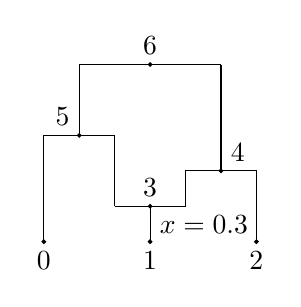
\begin{tikzpicture}[scale=0.45]

    \draw (-2,0) -- (-2,3) -- (0, 3);
    \draw (1,0) -- (1,1);
    \draw (0,1) -- (2,1) -- (2,2) -- (4,2) -- (4,0);
    \draw (3,2) -- (3,5);
    \draw (0,1) -- (0,3);
    \draw (-1, 3) -- (-1, 5) -- (3,5);

    \draw[fill] (-2,0) circle [radius=0.05];
    \draw[fill] (-1,3) circle [radius=0.05];
    \draw[fill] (1,0) circle [radius=0.05];
    \draw[fill] (4,0) circle [radius=0.05];
    \draw[fill] (1,1) circle [radius=0.05];
    \draw[fill] (3,2) circle [radius=0.05];
    \draw[fill] (1,5) circle [radius=0.05];

    \node [below] at (-2,0) {0};
    \node [below] at (1,0) {1};
    \node [below] at (4,0) {2};
    \node [above] at (1,1) {3};
    \node [below right] at (1,1) {$x = 0.3$};
    \node [above right] at (3,2) {4};
    \node [above left] at (-1,3) {5};
    \node [above] at (1,5) {6};

    \end{tikzpicture}
% \begin{center}
% $\equiv$
% \end{center}
% \end{column}
% \begin{column}{5cm}
\includegraphics[width=3.8cm]{illustrations/arg-ts.pdf}
\includegraphics[width=3.8cm]{illustrations/arg-ts-simplified.pdf}
\includegraphics[width=3.8cm]{figures/arg.pdf}

\end{center}
\caption{\label{fig-arg} (A) An simple ARG in which a recombination
occurs at position 0.3; (B) the equivalent topology depicted as a tree
sequence, including the recombination node; (C) the same tree sequence
topology ``simplified'' down to its minimal tree sequence representation;
(D) the fraction of nodes in a tree sequence that are concerned with
extra ARG information in a tree sequences returned using \msprime's
\texttt{record\_full\_arg} mode}
\end{figure}

However, this original definition of the ARG in terms of a stochastic process
is rarely what is meant when the term is currently used. The term has come to
essentially mean any representation of genetic ancestry in the presence
of recombination as a graph-like structure; for example,
\cite{mathieson2020ancestry} informally define an ARG as the subset of an
individual's pedigree from which they have inherited ancestral material.
Others state that an ARG is equivalent to the sequence of marginal
% Also SARGE paper
trees along the genome~\citep{yang2016rapidly,mirzaei2016rent}

Such
imprecision is unfortunate, since there are any number of graphical encodings of
genetic ancestry, and referring to the original Griffiths papers does little to
clarify. As we see below, there are situations in which the precise information
stored in the graph is important, and conflating a high-level
discussion of genetic ancestry with this mathematical object is not
helpful. The point of technical terms is to provide clarity and
precision on what is being discussed, and it is now essentially
impossible to know what is meant by the term ``ARG'';
we therefore use the term ``genetic ancestry'' in high-level
discussions.

For our purposes, an ARG is a realisation of the coalescent with
recombination, in the Griffiths (little ARG) sense.
As described in detail by~\cite{kelleher2016efficient}, Hudson's algorithm
works by dynamically generating and traversing a little ARG.
The graph is not explicitly represented in memory, but is partially
present through the extant lineages and the ancestral material they carry
over time. Since the ARG is a large and unwieldy object
(Fig.~\ref{fig-arg}) we do not use it as output, but
rather store the information required to recover the genealogical
history as nodes and edges in a tree sequence (see section XX),
or ``coalescence records'' in the terminology of~\citep{kelleher2016efficient}.

Although the tree sequences output by \msprime\ contain full information
about the genealogical trees, their correlation structure along the genome,
and the ancestral haplotypes on which coalescences occured, some information
is lost in this mapping down from ARG space to the minimal tree sequence
form. In particular, we lose
information about ancestral haplotypes that were common ancestors but
in which no coalescences occured, and also information about the precise time
and genomic location of recombination events. In most cases, such
information is of little relevance as it is in principle unknowable,
but there are occasions such as visualisation or computing likelihoods (see
below) in which is useful. We therefore provide
the \texttt{record\_full\_arg} option in \msprime\
to store a representation of the complete ARG traversed during simulation.
This is done by storing extra nodes (marked with specific flags, so they
can be easily identified later) and edges in the tree sequence.
Fig.~\ref{fig-arg} shows that this extra ARG information
quickly comes to dominate the output as we increase the sequence length,
and the resulting tree sequence files are many times larger
than the standard minimal tree sequence representation.

One situation in which a record of the full ARG is necessary is when we
wish to compute likelihoods during inference.
The likelihood is a central quantity in evaluating the plausibility of a putative
ancestry as an explanation of DNA sequence data, both directly through
e.g.~approaches based on maximum likelihood, and as an ingredient of
methods such as
Metropolis-Hastings~\citep{kuhner2000maximum,nielsen2000estimation,wang2008bayesian}.
We provide functions to compute the likelihood of ARG realisations
(encoded using the representation of the \texttt{record\_full\_arg} option)
and mutational patterns under
the standard coalescent and infinite sites mutation model.
See the Appendix for details.

\subsection*{Selection}
\label{sec-selection}
Another ellaboration of the standard neutral coalescent with recombination
is the addition of selective sweeps~\citep{kaplan1989hitchhiking,braverman1995hitchhiking,kim2002detecting}.
In the context of the coalescent this amounts to creating a structured population
during the sojourn of the beneficial mutation through the population (i.e., the sweep phase)
in which lineages may transit between favored and unfavored backgrounds through
recombination. This allows for many selective sweep scenarios, including recurrent, partial,
and soft selective sweeps to be simulated efficiently, however in general this
efficiency comes at the cost of flexibility in comparison to forwards in
time simulation.

Currently there are a small number of other simulators that will generate
coalescent samples with sweeps including, SelSim~\citep{spencer2004selsim}
mbs~\citep{teshima2009mbs}, msms~\citep{ewing2010msms},
Cosi2~\citep{shlyakhter2014cosi2}, and discoal~\citep{kern2016discoal}.
Each of these packages has their own benefits and possible drawbacks,
however none of them at present will output tree sequence formatted data.

\begin{figure}
\begin{center}
\includegraphics[width=6cm]{figures/sweeps-perf}
\end{center}
\caption{\label{fig-selection-perf}Comparison of the runtime for
\msprime\ and \texttt{discoal} for simulating selective sweeps.
}
\end{figure}

We have implemented selective sweeps in \msprime\ similarly to
the \texttt{discoal} implementation-- sweep trajectories are
generated from a jump process approximation to the conditional diffusion
of an allele bound for fixation~\citep{coop2004ancestral}.
This implementation allows us to further generalize sweep models to
changing population sizes as well as selection from standing variation,
both of which are features that are planned for the near future.
Moreover because this implements the basic infrastructure for the structured
coalescent, adding support for, e.g.,
inversions is straightforward~\citep{peischl2013sequential}.

\subsection*{Discrete time Wright-Fisher}

The assumptions of the classical coalescent model are that both sample size and
the simulated sequence length are small. As modern datasets often include
whole-genome sequences for tens or hundreds of thousands of samples, simulating
such data requires breaking these assumptions. While the coalescent remains a
good approximation to the Wright-Fisher model in the distant past, it can
exhibit large biases in the recent history. Identity-by-descent (IBD),
long-range linkage disequilibrium (LD), and ancestry patterns deviate from
Wright-Fisher expectations, and this bias grows considerably when simulating
larger sample
sizes~\citep{wakeley2012gene,bhaskar2014distortion,nelson2020accounting}.

A backwards-in-time Wright-Fisher model is supported in \msprime, which is
shown to properly capture the expected distributions of IBD and long-range LD,
as well as ancestry patterns in admixed
populations~\citep{nelson2020accounting}. In short, the classical coalescent
draws recombination events from exponential waiting times, which are continuous
in time, and each recombination then splits a segment into two distinct
ancestors. For large sequence lengths, this can dramatically overestimate the
number of genealogical ancestors of a given sample. Instead, the Wright-Fisher
model iterates through discrete generations so that each gamete has a unique
diploid parent, and multiple recombinations within a generation results in
crossover events between the same two parental haploid copies.  This method is
described in more detail in~\cite{nelson2020accounting}.

\begin{figure}
\begin{center}
\includegraphics[width=6cm]{figures/dtwf-perf}
\end{center}
\caption{\label{fig-dtwf-perf} Comparison of \msprime's DTWF
simulations with ARGON. To ensure the comparison with ARGON is
as fair as possible we run it with a mutation rate of 0 and with
the minimum output options (so that it writes out only an empty VCF file)}
\end{figure}

We support changing the simulation model at specified times so that we can
easily run hybrid simulations, as proposed by~\cite{bhaskar2014distortion}. We
can combine any number of different simulation models, allowing for the
flexible choice of simulation scenarios without severely damaging efficiency.
As the discrete time Wright-Fisher model improves accuracy of genealogical
patterns in the recent past, we can simulate the recent history using this
model and then switch to the standard coalescent to more efficiently simulate
the more ancient history. Fig.~\ref{fig-dtwf-perf} compares the perfomance of
this approach with ARGON~\citep{palamara2016argon}, a specialised DTWF
simulator.  The Wright-Fisher approach in \msprime\ is more efficient at
simulating chromosome-scale sequences (larger than $\approx10$Mb), while the
hybrid approach provides large efficiency gains.


\subsection*{Simulation interface}
\label{sec-sim-interface}

The majority of simulation packages are controlled either through
a command line interface~\citep[e.g.][]{hudson2002generating,kern2016discoal},
a text-based input file
format~\citep[e.g.][]{guillaume2006nemo,excoffier2011fastsimcoal,shlyakhter2014cosi2},
or a mixture of both.
Command line interfaces such as \ms\ make it very easy to run simple
simulations, but as model complexity and the number of parameters specified increases
they become difficult to understand and
error-prone~\citep{ragsdale2020lessons,gower2021demes}.
Specifying parameters through a text file alleviates this problem to a degree,
but lacks flexibility, for example, when running simulations with parameters
drawn from some distribution. In practice, for any significant simulation
project (or at least, any reproducible one), users will write a script
to generate the required command lines or input parameter files,
invoke the simulation engine, and process the results in some way.
This process is cumbersome and labour intensive, and
a number of packages have been developed
to allow simulations be run directly in a high-level
scripting language~\citep{staab2016coala,parobek2017skelesim,gladstein2018simprily}.

The more recent trend has been to move away from this file and command-line
driven approach and to instead provide direct interfaces to the simulation
engines via an Application Programming Interface (API)~\citep[e.g.][]{
thornton2014cpp,kelleher2016efficient,becheler2019quetzal,haller2019slim}.
The primary interface for \msprime\ is through a thoroughly documented and
stable Python
API, which has allowed a number of downstream tools to be built on top of
% Found these through the Dependent packages on GitHub
it~\citep{terhorst2017robust,chan2018likelihood,spence2019inference,
adrion2020community,adrion2020predicting, kamm2020efficiently,
mckenzie2020ipcoal, montinaro2020revisiting,
de2021geonomics,rivera2021simulation}.
As well as providing a stable and efficient platform for building
downstream applications, \msprime's Python API makes it much easier to
build reproducible simulation pipelines, as the entire workflow can
be encapsulated in a single script, and package and version
dependencies can be explicitly stated using the \texttt{pip}
or \texttt{conda} package managers.
For example, the errors made~\citep{ragsdale2020lessons,martin2020erratum}
in the influential simulation analysis of
\cite{martin2017human} were only detected because the pipeline
could be easily run and reanalysed.

A major change for the \msprime\ 1.0 release is the introduction of a new set of APIs,
designed in part to avoid sources of error (see the Demography section) but
also to provide more appropriate defaults while keeping compatibility with
existing code. In the new APIs, ancestry and mutation simulation are fully
separated, with the \texttt{sim\_ancestry} and \texttt{sim\_mutations}
functions replacing the legacy \texttt{simulate} function. Among other changes,
the new APIs default to discrete genome coordinates and finite sites mutations,
resolving a major source of confusion and error. The 0.x APIs are fully
supported and tested, and will be maintained for the foreseeable future.
We also provide an \ms\ compatible
command line interface to support existing workflows, and the
\texttt{msp} program that supports specifying demographic models in
Demes format~\citep{gower2021demes} from the command line.


\subsection*{Development model}
The community development process for \msprime\ is enabled by following an
open source development practise with a strong emphasis on code quality
and correctness. To ensure a consistent style, we require that all code
follows the PEP8 guidelines. Unit tests for all additions are required, and
are automatically run on each pull request on a variety of continuous
integration testing platforms. For new simulation features, statistical tests
must also be added, comparing the distribution of results to either analytical
results or existing simulators.

\section*{Discussion}
% Simulation is useful, and it's really easy for a single locus.
% This has lead to a culture of developing lots of simulators
% rather than focusing on one
Simulation has played a key role in the development of coalescent theory
and its use in understanding observed patterns of genetic variation.
The basic model can be simulated for $n$ samples in $O(n)$ time
and is straightforward to implement---for example, Hudson provided a fully
functional and highly efficient simulator as a C source code listing in an
appendix to the seminal review paper~\citep{hudson1990gene}. Because of
this ease, the dominant approach to producing simulators for extensions
to this basic model has been to develop them independently. This is
often seen as a learning opportunity, since those developing extensions
to the coalescent must have an excellent understanding of the basic
model in order to develop extensions to the coalescent.
The coalescent with recombination, however, is \emph{not} straightforward
to implement, and numerous different approaches have been
proposed over the
years~\citep{hudson1983properties,griffiths1997ancestral,wiuf1999recombination,
mcvean2005approximating}. It has only recently become clear that it is
possible to implement the model efficiently, and only through the use
of sophisticated data structures and
intricate algorithms~\citep{kelleher2016efficient}.

% Making lots of simulators has given us a fragmented and poor
% quality ecosystem.
The approach of developing ``in-house'' simulators
has lead to a huge proliferation of different programs, with
slightly different feature sets and often incompatible interfaces.
It is a fragmented ecosystem with significant issues with software
quality (see, e.g.,~\cite{yang2014critical}),
and few simulators are actively maintained after publication.
We have seen that \msprime\ (for larger samples at least)
has at worst comparable, but usually far superior
performance to more specialised methods.

% JK: I want to make the point that the established idea that
% developing your own simulation software is a good learning experience
% is pretty questionable these days, and tends to produce a lot of
% crappy unmaintained software. Not sure if the following paragraph
% does the job that well, though.

There seems to be little point in continuing the huge duplication of effort we
have seen. It is not possible to achieve the performance levels of \msprime\
without investing substantially in software engineering. As demonstrated here,
\msprime\ is extensible and we would argue that developing this simulator as an
open-source community asset is of more benefit to all. Implementing a
coalescent simulator may once have been a good way for (e.g.) a student to
learn about programming and simulation, but it is no longer reasonable to
expect this. There is simply too much engineering required. For example, as of
the 1.0.0 release \msprime\ consisted of around 13K lines of C and 11K
lines of Python, with test suites of 122 C test cases (7K lines of code) and
1350 Python test cases (22K lines of code), along with a suite of 217
statistical validation tests (6K lines of code). It requires a sustained effort
over years to produce well engineered, high-quality software. It may reasonably
be asked if students would learn more from contributing to an existing project
with established high-quality engineering standards, or from producing their own
software in a self-taught manner.

A significant advantage to simulating the coalescent with recombination
backwards in time using Hudson's algorithm rather than
left-to-right
approaches~\citep{wiuf1999recombination,chen2009fast,staab2015scrm}
is the ease with which additional processes can be integrated.
We have seen that processes such as gene conversion, complex
demography, instantaneous bottlenecks, multiple merger caolescents
and selective sweeps have been integrated seamlessly into
the simulations. Incorporating any of these extensions into
either the exact or approximate left-to-right processes would require
complex derivations. Because we are going backwards
in time, processes can be modelled as competing exponentials
using Gillespie's algorithm \jkcomment{I think?},
and therefore in principle we can
add as many extra processes as we like.
\jkcomment{so, backwards in time
sims in msprime is extensible for the future.}


There is also the welcome development of libraries such as
Quetzal~\citep{becheler2019quetzal} and libsequence~\citep{thornton2014cpp}
which break this pattern of monolithic simulation software.


Thus, development of \msprime\ is not completed and much remains
to be done.

Tskit has facilited unprecedented interoperability between simulators:
Forward simulations can also use tree
sequences~\citep{kelleher2018efficient,haller2018tree}. In particular, SLiM
3.0~\citep{haller2019slim} and fwdpp~\citep{thornton2014cpp} can now output
tree sequences. Msprime can take tree sequences simulated by these forward
simulators as input and complete the simulation (``recapitation'').
See \cite{haller2018tree} for more details.



% Finish up with a paragraph saying that there loads of exciting
% new things that simulation can do. We need MORE sims!!!
The ability to infer trees at scale for the first time
in the presence of
recombination~\citep{harris2019database,kelleher2019inferring,
speidel2019method,tang2019genealogy}
% also SARGE
opens the possibility for new applications of coalescent simulations.
With lots of applications, e.g., [cite Osmond and Coop].
Also \stdpopsim\ is cool~\citep{adrion2020community}

\section*{Acknowledgments}
JK is supported by the Robertson Foundation.
Jere Koskela is supported in part by EPSRC grant EP/R044732/1.
ADK was supported by NIH awards R01GM117241 and R01HG010774.
Franz Baumdicker is funded by the Deutsche Forschungsgemeinschaft
EXC 2064/1 -- Project number 390727645, and EXC 2124 -- Project number 390838134.

\bibliographystyle{plainnat}
\bibliography{paper}


%% local definitions for section multiple merger coalescents
 \newcommand{\be}{\begin{equation}}
 \newcommand{\ee}{\end{equation}}
 \newcommand{\bd}{\begin{displaymath}}
 \newcommand{\ed}{\end{displaymath}}
\newcommand{\IN}{\ensuremath{\mathds{N}}}%
\newcommand{\EE}[1]{\ensuremath{\mathds{E}\left[ #1 \right]}}%
\newcommand{\one}[1]{\ensuremath{\mathds{1}_{\left\{ #1 \right\}}}}%
\newcommand{\prb}[1]{\ensuremath{\mathds{P}\left( #1 \right) } }%

\NewEnviron{esplit}[1]{%
\begin{equation}
\label{#1}
\begin{split}
  \BODY
\end{split}\end{equation}
}

\setcounter{secnumdepth}{2} % Print out appendix section numbers

\appendix

\section*{Theoretical runtime}
    \label{app-theoretical-runtime}

\begin{figure}
\begin{center}
    \includegraphics{figures/ancestry-perf-expected}
\end{center}
\caption{\label{fig-expected-perf}
    Data from Figure~\ref{fig-ancestry-perf}, compared with
    equation~\eqref{eqn-hsw-bound} (``expected'').
    Left panel shows observed times plotted against expected number
    of operations; right panel shows the ratio of the two, plotted against $\rho$.
}
\end{figure}

The book \citet{hein2004gene} (Equation 5.10) gives a theoretical upper bound
on the number of events involving trapped ancestral material in Hudson's algorithm.
For $n$ samples from 
a diploid population of effective size $N_e$,
and a genome of genetic length $r$,
with $\rho = 4 N_e r$ the scaled recombination rate,
and $R^T$ the number of recombination recombination events in trapped material,
this upper bound is
\begin{equation} \label{eqn-hsw-bound}
    \mathbb{E}[R^T]
    \le
    \rho (\rho + 1) \left( \sum_{i=1}^{n-1} \frac{1}{i} \right)^2 .
\end{equation}
Note that the sum on the right is well-approximated by $\log(n)$.
Although \citet{hein2004gene} refer to this bound as ``crude'',
it turns out to predict the scaling of runtime quite well for large genomes.
Figure~\ref{fig-expected-perf} shows the observed runtime
(from the same simulations as Figure~\ref{fig-ancestry-perf})
plotted against equation~\eqref{eqn-hsw-bound},
showing that for values of $\rho$ above $4 \times 10^4$ or so
(i.e., chromosome-length simulations in populations above $10^4$),
the ratio of observed time to the value from \eqref{eqn-hsw-bound} is constant.
This implies the runtime for a large sample
can be predicted from the runtime for a small sample.
For smaller values of $\rho$, however, the prediction
severely underestimates runtime.


\section*{Mutation generation}
\label{app-mutation-algorithm}

The algorithm that \msprime\ uses to simulate mutations on a tree sequence
proceeds in two steps:
first, mutations are ``placed'' on the tree sequence
(i.e., sampling their locations in time, along the genome, and on the marginal tree),
and then the ancestral and derived alleles of each mutation are generated.
All mutation models share the code to place mutations,
but choose alleles in different ways.

First, mutations are placed on the tree sequence under an inhomgeneous Poisson model
by applying them independently to each edge.
If an edge spans a region $[a, b)$ of the genome
and connected parent and child nodes with times $s < t$,
and the mutation rate locally is $\mu$,
then the number of mutations on the edge is Poisson with mean $\mu (t-s) (b-a)$,
and each mutation is placed independently at a position chosen uniformly in $[a,b)$
and a time uniformly in $[s,t)$.
In a discrete genome, all positions are integers and so more than one mutation
may occur at the same position on the same edge.
Otherwise (i.e., for an infinite-sites model),
positions are rejection sampled to obtain a unique floating-point number.
If an edge spans a region of the genome with more than one mutation rate,
this is done separately for each distinct region.
The algorithm scales with the number of edges in the tree sequence.
Since the number of edges is proportional to the number of marginal trees,
this is equivalent to an algorithm that applies mutations separately
to each marginal tree,
but avoids the bookkeeping necessary to place mutations uniformly on a tree
(as opposed to drawing locations uniformly on the box $[a,b) \times [s, t)$
as we do here).

Next, alleles are chosen for each mutation.
If the site was not previously mutated, then a new ancestral allele is chosen for the site.
Then, each mutation on the tree is considered in turn,
in decreasing order of time ago,
and a derived allele is chosen based on the parental allele
(which may be the ancestral allele or the derived allele of a previous mutation)
and some randomness.
Finally, information about the mutations are recorded in the site and mutation tables
of the tree sequence.

A mutation model must, therefore, provide two things:
a way of choosing an ancestral allele for each new variant site,
and a way of choosing a derived allele given the parental allele at each mutation.
Perhaps the simplest mutation model implemented in \msprime\ is the
\texttt{InfiniteAlleles} mutation model,
which keeps an internal counter so that the requested alleles are 
assigned subsequent (and therefore unique) integers.

Since the algorithm above applies mutations at a single rate
independent of ancestral state,
a model in which different alleles mutate at different rates
must necessarily produce some silent mutations.
To illustrate this, consider a mutation model on the binary alphabet
$\{X, Y\}$ in which $X$ mutates to $Y$ at rate $\alpha$
and $Y$ mutates to $X$ at rate $\beta$, with $\beta < \alpha$.
To implement this, first place mutations at the largest total rate, which is $\alpha$.
Then, at each site, choose an ancestral allele from the ``root distribution''
(a natural choice would be to choose from the stationary distribution,
$X$ with probability $\beta / (\alpha + \beta)$),
and for each mutation, choose a derived allele as follows:
if the parental allele is $X$, then choose $Y$;
if the parental allele is $Y$, then choose $X$ with probability $\beta/(\alpha + \beta)$,
and choose $Y$ otherwise.
This produces the correct distribution by Poisson thinning:
a Poisson process with rate $\alpha$ in which each point is discarded independently
with probability $\beta / (\alpha + \beta)$ is equivalent to a Poisson
process with rate $\beta$.
All finite-state models (implented under the generic \texttt{MatrixMutationModel} class)
work in this way: mutations are placed at the maximum mutation rate,
and then some silent mutations will result.

In previous versions of \msprime, silent mutations were disallowed,
and we could have removed them from the output entirely.
However, we have chosen to leave them in, so that for instance
simulating with the \texttt{HKY} mutation model will result in silent mutations
if not all equilibrium frequencies are the same.
Although the presence of silent mutations may at first be surprising
(although they don't affect calculations of statistics in any way),
there is a good reason to leave them in:
to allow layering of different mutation models.
Suppose that we wanted to model the mutation process as a mixture of more than one model,
e.g., Jukes-Cantor mutations at rate $\mu_1$, and
HKY mutations occur at rate $\mu_2$.
Layering multiple calls to \texttt{sim_mutations} is allowed,
so we could first apply mutations with the \texttt{JC69} model at rate $\mu_1$
and then add more with the \texttt{HKY} model at rate $\mu_2$.
However, there is a small statistical problem:
suppose that after applying Jukes-Cantor mutations we have an $A \to C$ mutation,
but then the HKY mutations inserts another mutation in the middle,
resulting in $A \to C \to C$.
If neither mutation model allows silent transitions,
then this is clearly not correct,
i.e., it is not equivalent to a model that simultaneously applies the two models.
(The impact is small, however, as it only affects sites with more than one mutation.)
The solution is to make the Jukes-Cantor model \emph{state-independent}
(also called ``parent-independent''),
by placing mutations at rate $4/3 \mu_1$ and then choosing the derived state for each mutation
\emph{independently} of the parent (so that 1/4 of mutations will be silent).
If so -- and, more generally, if the first mutational process put down is state-independent --
then the result of sequentially applying the two mutation models
is equivalent to the simultaneous model.
To facilitate this, many mutation models have a \texttt{state\_independent} option
that increases the number of silent mutations
and makes the model closer to state-independent.


\section*{Likelihood calculations}
\label{app-likelihoods}

We provide two functions to facilitate likelihood-based inference.
Both are implemented only for the simplest case of the standard ARG with a
constant population size, and require tree sequences compatible with the
\texttt{record\_full\_arg} option as their arguments.
\begin{itemize}
\item \texttt{msprime.log\_arg\_likelihood(ts, r, N)} returns the natural logarithm of
the sampling probability of the tree sequence \texttt{ts} under the ARG with per-link,
per-generation recombination probability \texttt{r} and population size \texttt{N}.
Specifically, the function returns the logarithm of
\begin{equation*}
\Bigg( \frac{ 1 }{ 2 N } \Bigg)^{ q_c } \Bigg( \prod_{ i : \mathcal{R} } r g_i \Bigg)
	\exp\Bigg( -\sum_{ i = 1 }^q \Big[\frac{ 1 }{ 2 N } \binom{ k_i }{ 2 }
		+ r l_i \Big] t_i  \Bigg),
\end{equation*}
where $t_i$ is the number of generations between the $(i - 1)$th and $i$th event,
$k_i$ is the number of extant ancestors in that interval, $l_i$ is the number of links
in that interval that would split ancestral material should they recombine,
$q$ is the total number of events in the tree sequence $\texttt{ts}$,
$q_c$ is the number of coalescences, $\mathcal{R}$ is the set of indices
of time intervals which end in a recombination, and $g_i$ is the corresponding
\emph{gap}:  the length of material in which the recombination at the end of the
$i$th period could have taken place without affecting the resulting genealogy.
A recombination in ancestral material will always have $g_i = 1$, while a recombination
in trapped non-ancestral material can result in other values of $g_i$.
For a continuous model of the genome and a recombination in ancestral material,
we set $g_i = 1$ and interpret the result as a density.
\item \texttt{msprime.unnormalised\_log\_mutation\_likelihood(ts, m)} returns the
natural logarithm of the probability of the mutations recorded in the tree sequence
\texttt{ts} given the corresponding ancestry, assuming the infinite sites model, up to
a normalising constant which depends on the pattern of mutations,
but not on the tree sequence or the per-site, per-generation mutation
probability \texttt{m}.
Specifically, the function returns the logarithm of
\begin{equation*}
e^{ - T m / 2 } \frac{ ( T m / 2 )^M }{ M ! }
\prod_{ \gamma \in \mathcal{ M } } \frac{ h_{ \gamma } }{ T },
\end{equation*}
where $T$ and $\mathcal{M}$ are the total branch length and set of mutations
in \texttt{ts}, respectively, and for a mutation $\gamma$, $h_{ \gamma }$ is the
total branch length on which $\gamma$ could have arisen while appearing on all
of the leaves of \texttt{ts} it does, and on no others.
Unary nodes on marginal trees arising from the \texttt{record\_full\_arg} option
mean that, in general $h_{ \gamma }$ corresponds to the length of one or more
edges.
\end{itemize}


\label{app-multiple-mergers}
\section*{Multiple merger coalescent model}

Multiple-merger coalescents, in which a random number of ancestral
lineages may merge at a given time in one group, and only one such
group of lineages can merge at any given time (asynchronous multiple
mergers), are referred to as $\Lambda$-coalescents; the rate at which  a given group of $k$ lineages out of a total of  $b$ lineages merges  is given by ($a\ge  0$ constant)
\begin{equation}\label{lambdabk}
\lambda_{b, k} =  \int_0^1  x^{k-2}(1-x)^{b-k}\Lambda(dx) + a\one{k=2}, \quad 2 \le k \le b,
\end{equation}
where $\Lambda$ is a finite measure on the  (Borel subsets of)  unit interval without an atom at zero \citep{DK99,P99,S99}.    The  total rate  is given by
\be\label{lambdab}
 \lambda_{b} = \int_0^1 \left(1 - (1-x)^{b} - bx(1-x)^{b-1} \right)x^{-2}\Lambda(dx) + \binom{b}{2},
\ee
\citep{S99}  which can be useful in applications, in particular  provided the  antiderivative  can be explicitly identified.

A larger class of multiple-merger coalescents involving simultaneous
multiple mergers of distinct groups of ancestral lineages also exists
\citep{S00}. These are commonly referred to as $\Xi$-coalescents, and
can be shown to be the limits of ancestral processes derived from
population models incorporating diploidy (or more general polyploidy)
\citep{BBE13,blath2016site}, and certain models of selection \citep{DS04}.
To describe a general $\Xi$-coalescent let $\Delta$ denote the
infinite simplex \be\label{Delta} \Delta := \{ (x_1, \ldots ): x_1 \ge
x_2 \ge \cdots \ge 0, \sum_{j}x_j \le 1\}; \ee for any
$r \in \{1,2, \ldots\}$ let $k_1, \cdots, k_r \ge 2$, and
$b = s + k_1 + \cdots + k_r$ be the total number of blocks in a given
partition ($s = b - k_1 - \cdots - k_r$ is the number of blocks not
participating in the mergers at the given time).  The existence of
simultaneous multiple-merger coalescents was proved by \cite{S00}.
There exists a finite measure $\Xi$ on $\Delta$, with
$\Xi = \Xi_0 + a\delta_0$, the measure $\Xi_0$ has no atom at zero,
$a >0$ is fixed, and the rate at which one sees a given (simultaneous)
merger of ancestral lineages with merger sizes $k_1, \ldots, k_r$,
$s = n - k_1 - \cdots - k_r$, is given by
\begin{esplit}{xi}
  \lambda_{n; k_1, \ldots, k_r; s}  & = \int_\Delta  \sum_{\ell = 0}^s \sum_{\substack {i_1, \ldots, i_{r+\ell} = 1\\ \text{all distinct}} }^\infty  \binom{s}{\ell} x_{i_1}^{k_1} \cdots  x
_{i_{r}}^{k_r} x_{i_{r+1}} \cdots x_{i_{r+\ell}}\left(1 - \sum_{j=1}^\infty x_j \right)^{s-\ell} \frac{1}{ \sum_{j=1}^\infty x_j^2 } \Xi_0(dx)   \\
  & +  a\one{r=1, k_1 = 2}.
\end{esplit}%
The number of such $(k_1, \ldots, k_r)$ mergers is
\be\label{N}
    \mathcal{N}(b; k_1, \ldots, k_r ) = \binom{b}{k_1 \ldots k_r\, s} \frac{1}{ \prod_{j=2}^b\ell_j!  },
\ee
\citep{S00},   in particular  $\mathcal{N}(b;2) = b(b-1)/2$, and one can compute the total rate of a  $(k_1, \ldots, k_r)$ merger as
\be\label{lambdabkall}
      \lambda(n; k_1, \ldots, k_r)         =    \mathcal{N}(b; k_1, \ldots, k_r ) \lambda_{n; k_1, \ldots, k_r; s}.
\ee

The total rate is given by, with
$n\ge 2$ denoting the total  number of ancestral lineages,
\be
\label{Xilambdab}
\lambda_{n} = \int_\Delta \left(1 - \sum_{\ell = 0}^n \sum_{i_1 \neq
\cdots \neq i_\ell } \binom{n}{\ell} x_{i_1}\cdots x_{i_\ell}\left(1
- \sum_{i=1}^\infty x_i\right)^{n-\ell} \right)
\frac{1}{\sum_{j=1}^\infty x_j^2}\Xi_0(dx) + a\binom{n}{2} \ee
\citep{S00}.  Viewing coalescent processes strictly as mathematical
objects, it is clear that the class of $\Xi$-coalescents contains
$\Lambda$-coalescents as a specific example (i.e.\ allowing at most
one group of lineages to merge each time), and the class of
$\Lambda$-coalescents contain the Kingman-coalescent as a special
case.  However, viewed as limits of ancestral processes derived from
specific population models they are not nested, since one would
obtain $\Lambda$-coalescents when deriving coalescent processes from
haploid population models incorporating sweepstakes reproduction and
high fecundity, and $\Xi$-coalescents for diploid populations.  One
should therefore apply the models as appropriate, i.e.\
$\Lambda$-coalescents to data (e.g.\ mtDNA data) inherited in a
haploid fashion, and $\Xi$-coalescents to e.g.\ autosomal data
inherited in diploid or polyploid fashion \citep{blath2016site}.


In \msprime\ we have incorporated two examples of multiple-merger coalescents.
One is a diploid extension \citep{BBE13} of the haploid model of sweepstakes
reproduction considered by \cite{EW06}, which is a haploid Moran model adapted
to sweepstakes reproduction.  Let $N$ denote population size, and take $\psi
\in (0,1]$ to be fixed.  In every generation, with probability
$1-\varepsilon_N$ a single individual (picked uniformly at random) perishes,
and one of the surviving individuals (sampled uniformly at random) produces one
offspring; with probability $\varepsilon_N$ a total of $\lfloor \psi N \rfloor$
individuals perish, and of the remaining individuals a single individual
produces $\lfloor \psi N \rfloor -1 $ offspring.  Taking $\varepsilon_N =
1/N^\gamma$ for some $\gamma > 0$, \cite{EW06} obtain specific examples of
$\Lambda$-coalescents, where the $\Lambda$ measure in Eq.~\eqref{lambdabk} is a
point mass at $\psi$.  The simplicity of this model does allow one to obtain
some explicit mathematical results (see e.g.\
\cite{EF2018,Matuszewski2017,Der2012,Freund2020}). The model considered by
\cite{EW06} has also been applied in algorithms for simulating gene genealogies
within phylogenies \citep{zhu2015hybrid}. The specific model incorporated into
\msprime\ is the diploid version \citep{BBE13} of the model studied by
\cite{EW06}, which would be necessary in order to incorporate recombination.
In the model considered by \cite{BBE13}, a single pair of diploid individuals
contribute offspring in each generation, selfing is excluded, and each
offspring is assigned one chromosome from each parent. There are, therefore,
four parent chromosomes involved in each reproduction event, which can lead to
up to four simultaneous mergers.  Let \begin{esplit}{Cconst} C_{b; k_1, \ldots,
k_r;s } &= \frac{4}{\psi^2} \sum_{\ell = 0}^{s \wedge (4-r)} \binom{s}{\ell}
(4)_{r+\ell} (1-\psi)^{s-\ell }\left( \frac{\psi}{4} \right) ^{k_1 + \cdots +
k_r + \ell},  \\ \end{esplit} where  $C_{b; k_1, \ldots, k_r;s }$ corresponds
to the coalescence rate $ \lambda_{b;k_1, \ldots, k_r;s}$ (see Eq~\eqref{xi})
of a  $\Xi$-coalescent on  $(\psi/4, \psi/4, \psi/4, \psi/4, 0, \ldots)$. The
total merger rate (see Eq~\eqref{lambdabkall}) is then
\be\label{xidirlambdabk} \lambda(b;k_1, \ldots, k_r) = \mathcal{N}(b; k_1,
\ldots, k_r ) \left( \frac{c\psi^2/4}{ 1 +  c\psi^2/4}C_{b; k_1, \ldots, k_r;s
} + \frac{ \one{r=1, k_1 = 2} }{1 +  c\psi^2/4}  \right), \ee and the total
coalescence rate becomes \begin{esplit}{xilambdab} \lambda_b & =
\frac{c\psi^2/4}{1 +  c\psi^2/4}  \frac{4 }{\psi^2 } \left(1 - \sum_{\ell = 0
}^{b\wedge 4} \binom{b}{\ell} (4)_\ell \left( \frac{\psi}{4} \right)^\ell (1 -
\psi)^{b-\ell } \right) + \frac{1}{1 +  c\psi^2/4} \binom{b}{2}.  \\
\end{esplit} The interpretation of \eqref{xilambdab} is that with probability
$1/(1 + c\psi^2/4)$  a `small' reproduction event occurs, in which the parent
pair produce one  diploid offspring; with probability  $c\psi^2/4/(1 +
c\psi^2/4)$ a `large' reproduction event occurs, in which  the parent pair
produce  $\lfloor \psi N \rfloor$ offspring.


The other multiple-merger coalescent model incorporated in \msprime\ is derived
from an adaptation of the haploid population model considered by
\cite{schweinsberg03} to diploid populations \citep{BLS15}.  In the haploid
version, in each generation individuals independently produce random numbers of
juveniles, where the random  number of juveniles $(X)$ produced by a given
individual  has the stable law \be\label{jX} \lim_{k\to \infty} C k^\alpha
\prb{X \ge k} = 1 \ee with index $\alpha > 0$, and $C > 0$ is a normalising
constant.   One can interpret  Eq.~\eqref{jX} as  stating the form of the
probability distribution  for number of juveniles at least on the order of the
population size.     If the random  total number of juveniles $(S_N)$ produced
in this way is at least the population size $(N)$, then one samples  $N$
juveniles uniformly at random without replacement to form the next generation
of  reproducing individuals; if  $S_N < N$ one simply  carries on with  the
same  set of individuals.   However,   assuming  $\EE{X} > 1$, one can show
that $\prb{S_N < N}$ decays exponentially fast in $N$ \citep{schweinsberg03}.
If $\alpha \ge 2$ the ancestral process converges to the Kingman-coalescent; if
$1 \le \alpha < 2$ the ancestral process converges to a specific case of a
$\Lambda$-coalescent, where the $\Lambda$ measure in Eq.~\eqref{lambdabk} is
associated with the Beta$(2-\alpha, \alpha)$ probability distribution, i.e.\
\be\label{Fbeta} \Lambda(dx) = \one{0< x \le 1} \frac{1}{B(2-\alpha,\alpha)}
x^{1 - \alpha}(1-x)^{\alpha - 1}  dx, \ee where $B(2-\alpha,\alpha)$ is the
beta function $B(a,b) = \Gamma(a)\Gamma(b)/\Gamma(a+b)$, $a,b > 0$
\citep{schweinsberg03}.
This model has been adapted to diploid populations
by \cite{BLS15}, where  the resulting coalescent process
is a  four-fold $\Xi$-coalescent on  $(x/4, x/4, x/4, x/4, 0, 0, \ldots)$,
where $x$ is a random variate with  the Beta$(2-\alpha,\alpha)$ distribution.
The merger rate (see Eq.~\eqref{xi}) is then ($1 \le r \le 4$)
\be\label{xibeta} \lambda_{b;k_1, \ldots, k_r} = \sum_{\ell = 0}^{ (b -
k)\wedge (4-r) } \binom{b-k}{\ell} \frac{ (4)_{r+\ell} }{4^{k+\ell}}
\frac{B(k+\ell - \alpha, b-k-\ell + \alpha ) }{B(2-\alpha,\alpha)} \ee
\citep{blath2016site,BLS15}. The interpretation of Eq.~\eqref{xibeta} is  that the
random   number of diploid  juveniles each  diploid pair of parents  produces
is  governed by  the law in Eq.~\eqref{jX},   and   each diploid juvenile  is
assigned  one chromosome  from each parent (selfing is excluded).

The model in Eq~\eqref{jX} assumes that individuals can produce arbitrarily
large numbers of juveniles. Considering diploid juveniles, this assumption is
probably rather strong, since diploid juveniles are at least fertilised eggs,
and so it is reasonable to suppose that the number of juveniles surviving to
the  particular life stage we are modeling  cannot be arbitrarily large.  With
this in mind, we also consider an adaptation of the Schweinsberg model, where
the random number of juveniles $(X)$ produced by a   given parent pair  is
distributed according to \be\label{jtr} \prb{X=k} =   \one{1 \le k \le \phi(N)}
\frac{\phi(N+1)^\alpha }{ \phi(N+1)^\alpha - 1 }  \left( \frac{1}{k^\alpha} -
\frac{1}{(k+1)^\alpha}  \right) , \ee where $\phi(N)$ is a deterministic strict
upper bound on the number of juveniles produced by  any given parent pair (see
also \citep{Eldon2018}).   One can follow the calculations in
\citep{schweinsberg03} or \citep{BLS15}  to show  that  if $1 < \alpha < 2$
then  $(k = k_1 + \cdots + k_r)$ then the merger rate (see Eq.~\eqref{xibeta})
is
 \be \lambda_{b;k_1, \ldots, k_r} =  \sum_{\ell = 0}^{ (b - k)\wedge (4-r) }
\binom{b-k}{\ell} \frac{ (4)_{r+\ell} }{4^{k+\ell}} \frac{B(M; k+\ell - \alpha,
b-k-\ell + \alpha ) }{B(M;2-\alpha,\alpha)}
\ee
with $B(z;a,b) := \int_0^z
t^{a-1}(1-t)^{b-1}dt$ for  $a,b>0$ and $0< z\le 1$, and \be M :=  \frac{K}{K+m}
\one{\phi(N) = KN} + \one{\phi(N)/N \to \infty } \ee where $K > 0$ is a
constant and  $m := \lim_{N\to \infty} \EE{X} = 1 + 2^{1-\alpha}/(\alpha - 1)$
\citep{CDEE2020,AEKKZ2020}.    In other words,  the measure $(\Lambda)$ driving
the multiple mergers is of the same form as in Eq.~\eqref{Fbeta}  with $0 < x
\le M$ in the case $1 < \alpha < 2$ and $\phi(N) \ge KN$.   If $\alpha \ge 2$
or $\phi(N)/N \to 0$ then  the  ancestral process converges (in the sense of
convergence of  finite-dimensional distributions) to  the Kingman-coalescent
\citep{CDEE2020,AEKKZ2020}.

\begin{comment}%
A coalescent process is a continuous-time Markov process taking values among
the partitions of $\IN := \{1,2, \ldots \}$, such that the restriction to any
finite $n \in \IN $ takes values among partitions of $[n] := \{1, 2, \ldots,
n\}$.  Write $\one{A} = 1$ if $A$ holds, and zero otherwise.   Let $\cP_n$
denote the set of partitions of $[n]$.  In the classical Kingman-coalescent,
the only possible transitions are the mergers of pairs of blocks (elements of a
partition $\pi \in \cP_n$), one pair at a time.  The $n$ leaves (corresponding
to the sampled DNA sequences) are arbitrarily labelled from 1 to $n$, and  the
blocks of a partition represent the common ancestors of the labels of each
block.    The initial state is  (usually) taken as $\{ \{1\}, \ldots, \{n\}\}$,
and the final state, i.e.\ when the most recent common ancester is reached, as
$\{ [n]\}$. A block in a partition of $[n]$ represents an ancestor of the
leaves in the block, i.e.\ the block $\{i_1, \ldots, i_k\}$ in a given
partition of $[n]$ is an ancestor of the $k$ leaves $i_1, \ldots, i_k \in [n]$,
and the leaves  correspond to arbitrarily labelled DNA sequences in the sample.
\end{comment}




\end{document}
